\documentclass[]{book}
\usepackage{lmodern}
\usepackage{amssymb,amsmath}
\usepackage{ifxetex,ifluatex}
\usepackage{fixltx2e} % provides \textsubscript
\ifnum 0\ifxetex 1\fi\ifluatex 1\fi=0 % if pdftex
  \usepackage[T1]{fontenc}
  \usepackage[utf8]{inputenc}
\else % if luatex or xelatex
  \ifxetex
    \usepackage{mathspec}
  \else
    \usepackage{fontspec}
  \fi
  \defaultfontfeatures{Ligatures=TeX,Scale=MatchLowercase}
\fi
% use upquote if available, for straight quotes in verbatim environments
\IfFileExists{upquote.sty}{\usepackage{upquote}}{}
% use microtype if available
\IfFileExists{microtype.sty}{%
\usepackage{microtype}
\UseMicrotypeSet[protrusion]{basicmath} % disable protrusion for tt fonts
}{}
\usepackage[margin=1in]{geometry}
\usepackage{hyperref}
\hypersetup{unicode=true,
            pdftitle={JV InvenTeams Activity Guides},
            pdfauthor={Lemelson-MIT Program},
            pdfborder={0 0 0},
            breaklinks=true}
\urlstyle{same}  % don't use monospace font for urls
\usepackage{natbib}
\bibliographystyle{apalike}
\usepackage{longtable,booktabs}
\usepackage{graphicx,grffile}
\makeatletter
\def\maxwidth{\ifdim\Gin@nat@width>\linewidth\linewidth\else\Gin@nat@width\fi}
\def\maxheight{\ifdim\Gin@nat@height>\textheight\textheight\else\Gin@nat@height\fi}
\makeatother
% Scale images if necessary, so that they will not overflow the page
% margins by default, and it is still possible to overwrite the defaults
% using explicit options in \includegraphics[width, height, ...]{}
\setkeys{Gin}{width=\maxwidth,height=\maxheight,keepaspectratio}
\IfFileExists{parskip.sty}{%
\usepackage{parskip}
}{% else
\setlength{\parindent}{0pt}
\setlength{\parskip}{6pt plus 2pt minus 1pt}
}
\setlength{\emergencystretch}{3em}  % prevent overfull lines
\providecommand{\tightlist}{%
  \setlength{\itemsep}{0pt}\setlength{\parskip}{0pt}}
\setcounter{secnumdepth}{5}
% Redefines (sub)paragraphs to behave more like sections
\ifx\paragraph\undefined\else
\let\oldparagraph\paragraph
\renewcommand{\paragraph}[1]{\oldparagraph{#1}\mbox{}}
\fi
\ifx\subparagraph\undefined\else
\let\oldsubparagraph\subparagraph
\renewcommand{\subparagraph}[1]{\oldsubparagraph{#1}\mbox{}}
\fi

%%% Use protect on footnotes to avoid problems with footnotes in titles
\let\rmarkdownfootnote\footnote%
\def\footnote{\protect\rmarkdownfootnote}

%%% Change title format to be more compact
\usepackage{titling}

% Create subtitle command for use in maketitle
\newcommand{\subtitle}[1]{
  \posttitle{
    \begin{center}\large#1\end{center}
    }
}

\setlength{\droptitle}{-2em}
  \title{JV InvenTeams Activity Guides}
  \pretitle{\vspace{\droptitle}\centering\huge}
  \posttitle{\par}
  \author{Lemelson-MIT Program}
  \preauthor{\centering\large\emph}
  \postauthor{\par}
  \predate{\centering\large\emph}
  \postdate{\par}
  \date{2018-08-08}

\usepackage{booktabs}

\begin{document}
\maketitle

{
\setcounter{tocdepth}{1}
\tableofcontents
}
\chapter*{Preface}\label{preface}
\addcontentsline{toc}{chapter}{Preface}

Brief explanatory text about the program. Inventions
\citep{inventingModAm} are useful and unique.

\chapter{Chill Out}\label{chill-out}

\begin{center}
\includegraphics[width=0.5\linewidth]{img/chillOut} \end{center}

Unit overview text

\section{Educator Guide}\label{educator-guide}

Educator Guide version

\subsection*{What is Heat?}\label{what-is-heat}
\addcontentsline{toc}{subsection}{What is Heat?}

Lorem ipsum dolor sit amet, consectetur adipiscing elit, sed do eiusmod
tempor incididunt ut labore et dolore magna aliqua. Ut enim ad minim
veniam, quis nostrud exercitation ullamco laboris nisi ut aliquip ex ea
commodo consequat.

Duis aute irure dolor in reprehenderit in voluptate velit esse cillum
dolore eu fugiat nulla pariatur. Excepteur sint occaecat cupidatat non
proident, sunt in culpa qui officia deserunt mollit anim id est laborum.

\subsection*{Keep your Cool}\label{keep-your-cool}
\addcontentsline{toc}{subsection}{Keep your Cool}

Ullamcorper a lacus vestibulum sed arcu non odio euismod lacinia. Et
pharetra pharetra massa massa. Maecenas accumsan lacus vel facilisis
volutpat est velit egestas. Sit amet volutpat consequat mauris nunc
congue nisi vitae suscipit. Faucibus scelerisque eleifend donec pretium
vulputate sapien nec sagittis aliquam. Enim eu turpis egestas pretium.
Ut etiam sit amet nisl purus in mollis. A scelerisque purus semper eget
duis at. Fermentum dui faucibus in ornare quam. Sit amet purus gravida
quis blandit turpis cursus in hac. Ipsum consequat nisl vel pretium
lectus quam id leo. At auctor urna nunc id cursus metus aliquam
eleifend. Metus vulputate eu scelerisque felis imperdiet proin. Egestas
dui id ornare arcu. Ultricies mi eget mauris pharetra et ultrices neque
ornare. Sed libero enim sed faucibus turpis in eu mi bibendum. Massa
tincidunt dui ut ornare lectus sit amet est. Hendrerit dolor magna eget
est. Est pellentesque elit ullamcorper dignissim cras tincidunt
lobortis.

\subsection*{Removing Heat}\label{removing-heat}
\addcontentsline{toc}{subsection}{Removing Heat}

Lorem ipsum dolor sit amet, consectetur adipiscing elit, sed do eiusmod
tempor incididunt ut labore et dolore magna aliqua. Ut enim ad minim
veniam, quis nostrud exercitation ullamco laboris nisi ut aliquip ex ea
commodo consequat. Duis aute irure dolor in reprehenderit in voluptate
velit esse cillum dolore eu fugiat nulla pariatur. Excepteur sint
occaecat cupidatat non proident, sunt in culpa qui officia deserunt
mollit anim id est laborum.

\subsection*{Peltier Prototyping}\label{peltier-prototyping}
\addcontentsline{toc}{subsection}{Peltier Prototyping}

Ullamcorper a lacus vestibulum sed arcu non odio euismod lacinia. Et
pharetra pharetra massa massa. Maecenas accumsan lacus vel facilisis
volutpat est velit egestas. Sit amet volutpat consequat mauris nunc
congue nisi vitae suscipit. Faucibus scelerisque eleifend donec pretium
vulputate sapien nec sagittis aliquam. Enim eu turpis egestas pretium.
Ut etiam sit amet nisl purus in mollis. A scelerisque purus semper eget
duis at. Fermentum dui faucibus in ornare quam. Sit amet purus gravida
quis blandit turpis cursus in hac. Ipsum consequat nisl vel pretium
lectus quam id leo. At auctor urna nunc id cursus metus aliquam
eleifend. Metus vulputate eu scelerisque felis imperdiet proin. Egestas
dui id ornare arcu. Ultricies mi eget mauris pharetra et ultrices neque
ornare. Sed libero enim sed faucibus turpis in eu mi bibendum. Massa
tincidunt dui ut ornare lectus sit amet est. Hendrerit dolor magna eget
est. Est pellentesque elit ullamcorper dignissim cras tincidunt
lobortis.

\subsection*{Invention Extension}\label{invention-extension}
\addcontentsline{toc}{subsection}{Invention Extension}

Lorem ipsum dolor sit amet, consectetur adipiscing elit, sed do eiusmod
tempor incididunt ut labore et dolore magna aliqua. Ut enim ad minim
veniam, quis nostrud exercitation ullamco laboris nisi ut aliquip ex ea
commodo consequat. Duis aute irure dolor in reprehenderit in voluptate
velit esse cillum dolore eu fugiat nulla pariatur. Excepteur sint
occaecat cupidatat non proident, sunt in culpa qui officia deserunt
mollit anim id est laborum.

\section*{Appendix}\label{appendix}
\addcontentsline{toc}{section}{Appendix}

\subsection*{Invention Worksheet}\label{invention-worksheet}
\addcontentsline{toc}{subsection}{Invention Worksheet}

\subsection*{Certificate of
Achievement}\label{certificate-of-achievement}
\addcontentsline{toc}{subsection}{Certificate of Achievement}

\subsection*{Word Wall Words}\label{word-wall-words}
\addcontentsline{toc}{subsection}{Word Wall Words}

\subsection*{Education Standards}\label{education-standards}
\addcontentsline{toc}{subsection}{Education Standards}

\section{Student Guide}\label{student-guide}

Student Guide version

\chapter{Electronic Textiles}\label{electronic-textiles}

\begin{center}
\includegraphics[width=0.3\linewidth]{img/electronicTextiles} \end{center}

Unit overview text

\section{Educator Guide}\label{educator-guide-1}

Educator Guide version

\section{Student Guide}\label{student-guide-1}

Student Guide version

\chapter{Growing Green}\label{growing-green}

\begin{center}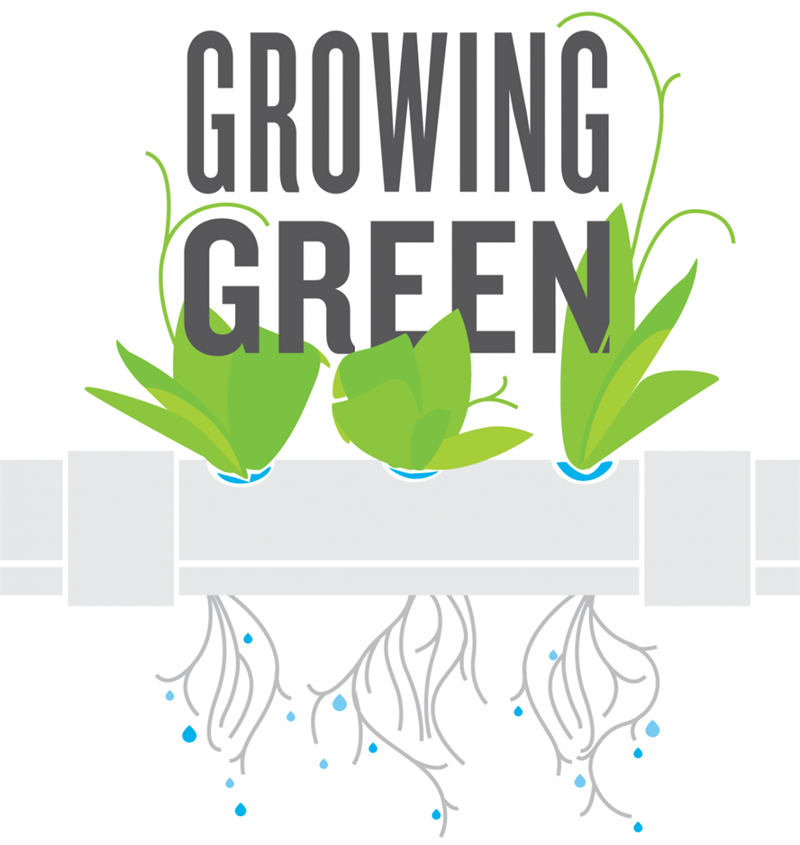
\includegraphics[width=0.5\linewidth]{img/growingGreen} \end{center}

Unit overview text

\section{Educator Guide}\label{educator-guide-2}

Educator Guide version

\section{Student Guide}\label{student-guide-2}

Student Guide version

\chapter{Noise Makers}\label{noise-makers}

\begin{center}
\includegraphics[width=0.5\linewidth]{img/noiseMakers} \end{center}

Unit overview text

\section{Educator Guide}\label{educator-guide-3}

Educator Guide version

\section{Student Guide}\label{student-guide-3}

Student Guide version

\chapter{Pump It Up}\label{pump-it-up}

\begin{center}
\includegraphics[width=0.5\linewidth]{img/pumpItUp} \end{center}

Unit overview text

\section{Educator Guide}\label{educator-guide-4}

Educator Guide version

\section{Student Guide}\label{student-guide-4}

Student Guide version

\chapter{Shoe Soles}\label{shoe-soles}

\begin{center}
\includegraphics[width=0.5\linewidth]{img/shoeSoles} \end{center}

Unit overview text

\section{Educator Guide}\label{educator-guide-5}

Educator Guide version

\section{Student Guide}\label{student-guide-5}

Student Guide version

\chapter{Super Lens}\label{super-lens}

\begin{center}
\includegraphics[width=0.5\linewidth]{img/superLens} \end{center}

Unit overview text

\section{Educator Guide}\label{educator-guide-6}

Educator Guide version

\section{Student Guide}\label{student-guide-6}

Student Guide version

\chapter{U Control}\label{u-control}

\begin{center}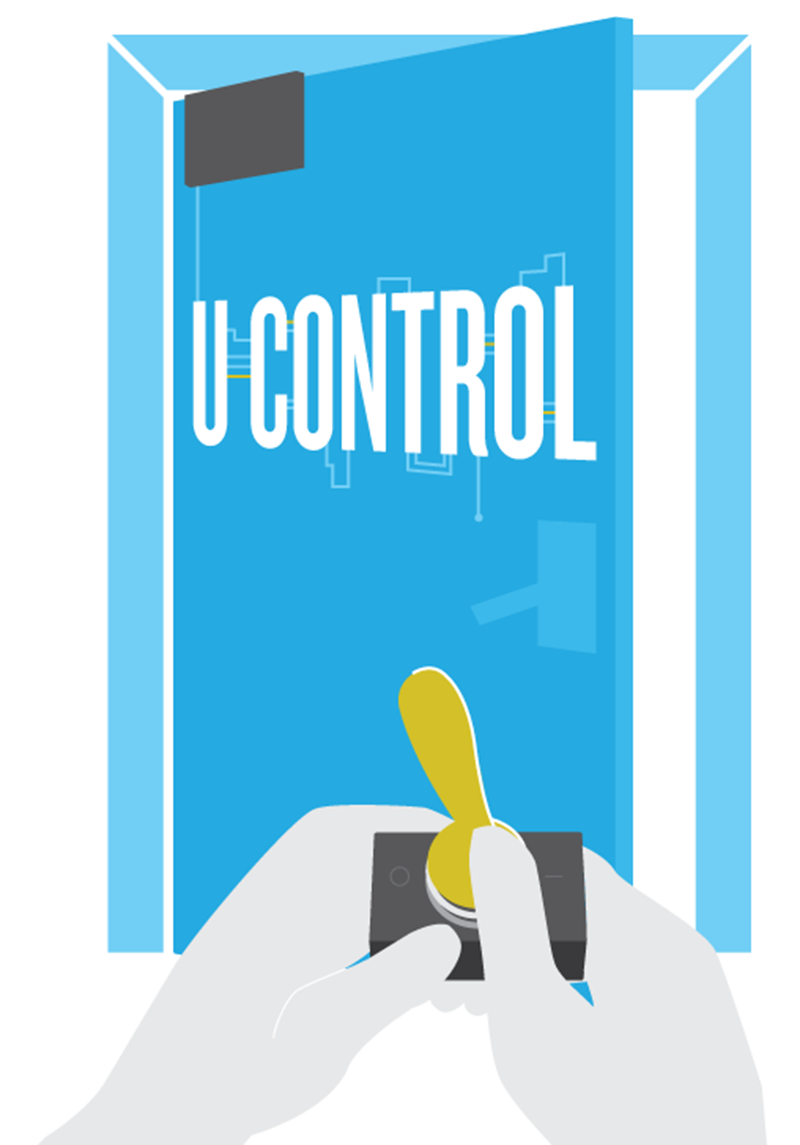
\includegraphics[width=0.5\linewidth]{img/uControl} \end{center}

Unit overview text

\section{Educator Guide}\label{educator-guide-7}

Educator Guide version

\section{Student Guide}\label{student-guide-7}

Student Guide version

\bibliography{book.bib}


\end{document}
